%%%%%%%%%%%%%%%%%%%%%%%%%%%%%%%%%%%%%%%%%%%%%%%%%%%%%%%%%%%%%
%%	Constitutive model form									%
%%%%%%%%%%%%%%%%%%%%%%%%%%%%%%%%%%%%%%%%%%%%%%%%%%%%%%%%%%%%%

\section{Effective constitutive model formulation}

%-----------------------------------------------------------
%	Kinematics
%-----------------------------------------------------------
\subsection{Kinematic considerations}
	
	The choice of kinematic basis is the first step to formulate constitutive models. Very often, it is useful to limit the choice of kinematic basis based on the available mechanical data or how well each basis match the response of the soft tissues, thus simplifying the form of the constitutive model and reducing parameter covariance during parameter estimation. However, for our approach, our aim is a highly generalized constitutive model that can match a wide range of possible micro-model responses using the same form, not restricting itself to the response and physics of specific soft tissue types. There is also no limitations to having sufficient mechanical data for parameter estimation, as this will be generated from the micro-models. As such, our considerations for choosing the kinematic basis are mainly:
\begin{enumerate}
    \item Most generalized form for reproducing a wide range of mechanical responses
    \item Simplest form for implementation and computational cost in numerical simulations
    \item Minimal number of parameters
    \item Minimal parameter covariance for parameter estimation
\end{enumerate}
    The smallest set of kinematic variables that can describe a wide range of soft tissues and deformations using the same simple form is ideal. 

    The invariants and pseudo-invariants of the right or left Cauchy Green tensor is very popular for the constitutive models of soft tissues. Indeed, we use them often with our structural models \cite{fata_insights_2014, zhang_meso_2016, avazmohammadi_novel_2017, sacks_novel_2016, zhang_modeling_2017}. There is a large number of invariants, each describes a facet of deformation: isotropic, volumetric strain, anisotropic, or interactions between them. The breadth of choices allow for more freedom in selecting a best combination when modeling specific soft tissues. However, there are simply too many invariants, and many of which are highly covariant. This does not lend itself for minimizing the number of parameters and the parameter covariance in a single fully generalized form. 
    
    
    It's here that using the components of the strain tensors is more practical for our approach. Although all strains are equivalent for constitutive modeling because they can be expressed with respect to each other, different strain tensors can have different effects when used directly in place of each other in the same form. For us, with the purpose of keeping the constitutive model form simple for implementation, the Green Lagrange strains are the most practical. Based on preliminary testing (Appendix \ref{sec:greenvshencky}), the Green Lagrange strains result in the simplest 2nd Piola Kirchhoff stress and elasticity tensor forms, and have behaviors that closely resemble the response of collagen fibers in soft tissues when under compression. We examined these aspects more closely in Appendix \ref{sec:greenvshencky}. 
    
    It is also convenient to express the Green Lagrange strain tensor with respect to the material axis (Fig. \ref{fig:greenkinematics}), $\mathbf{m}_0$, where
\begin{equation} \label{eqn:greenstrain}
E_m = \mathbf{m}_0\cdot\mathbf{E}\mathbf{m}_0, \quad E_n = \mathbf{n}_0\cdot\mathbf{E}\mathbf{n}_0, \quad E_{\phi} = \mathbf{m}_0\cdot\mathbf{E}\mathbf{n}_0,
\end{equation} 
    and $\mathbf{n}_0$ is the direction orthogonal to $\mathbf{m}_0$ (Fig. \ref{fig:greenkinematics}). This symmetry is helpful for further reducing the constitutive model form. 


%%%%%%%%%%%%%%%%%%%%%%%%%%%%%%%%%%%%%%%%%%%%%%%%%%%%%%%%%%%%
%-------------------	begin FIGURE 	-------------------%
\begin{figure}
\centering
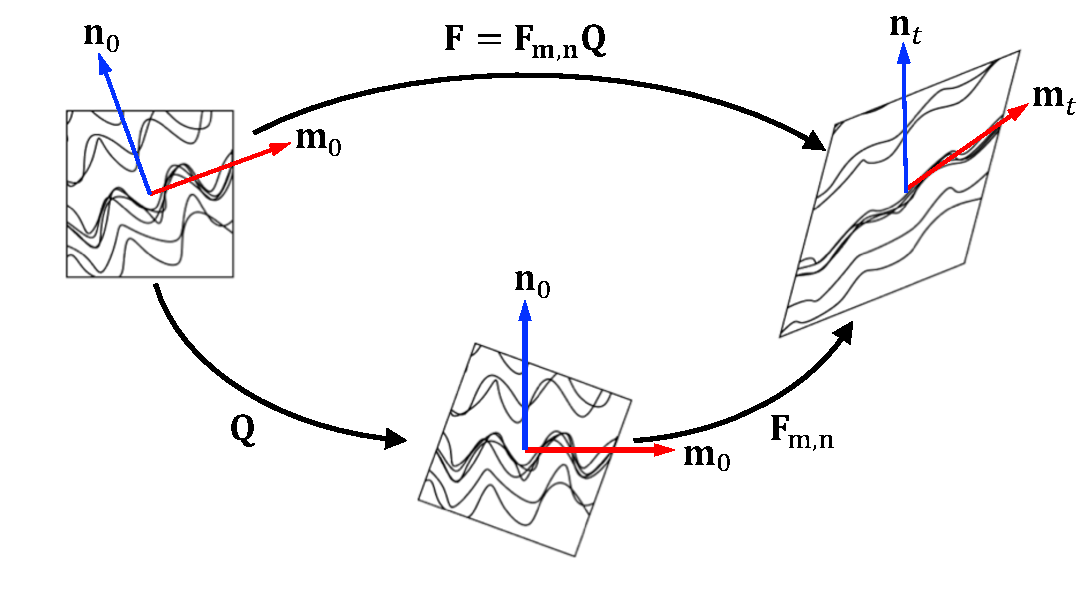
\includegraphics[width=5.0in]{Images/chapter5/greenkinematics.pdf}
\caption{By taking the right polar decomposition of the deformation gradient tensor, we can express the components of the Green Lagrange strain tensor with respect to the material axis. This creates a symmetry for the shear component of the Green Lagrange strain tensor, allowing us to further simplify the model form.}
\label{fig:greenkinematics}
\end{figure}
%-------------------	 end FIGURE 	-------------------%
%%%%%%%%%%%%%%%%%%%%%%%%%%%%%%%%%%%%%%%%%%%%%%%%%%%%%%%%%%%%












%-----------------------------------------------------------
%	Model formulation
%-----------------------------------------------------------
\subsection{Effective constitutive model form}
\subsubsection{Possible family of forms for the effective constitutive model}

    Using phenomenological approaches is necessary for minimal computational cost. The form of phenomenogical models for soft tissues generally falls into three families. The first family is composed of a summation of polynomials, 
%==========================================================%
%-------------------	begin EQUATION 	-------------------%
\begin{equation}
\begin{aligned}
\Psi	&= \sum_i\sum_j\sum_k c_{ijk}E_m^i E_n^j E_\phi^k. 
\end{aligned} \label{eqn:polynomialmodelform}
\end{equation}
%-------------------	 end EQUATION 	-------------------%
%==========================================================%
    We will refer to this family as the polynomial series approach. The second family is composed of separated exponential functions of individual or combinations of invariants or strains used, for example by Vito \textit{et al.} \cite{vito_mechanical_1980},
%==========================================================%
%-------------------	begin EQUATION 	-------------------%
\begin{align}\label{eqn:vitomodelforms}
\Psi 	&= \sum_i\sum_j\sum_k c_{ijk} e^{b_{ijk}E_m^i E_n^j E_\phi^k}.
\end{align}
%-------------------	 end EQUATION 	-------------------%
%==========================================================%
    We will refer to this family as the separated exponential approach. The final family is exponential models composed of a single exponential function of the sum of polynomials,
%==========================================================%
%-------------------	begin EQUATION 	-------------------%
\begin{equation}
\begin{aligned}\label{eqn:exponentialmodelform}
\Psi 	&= c_0 \left(e^{Q} - 1\right) \\
Q		&= \sum_i\sum_j\sum_k b_{ijk}E_m^i E_n^j E_\phi^k.
\end{aligned}
\end{equation}
%-------------------	 end EQUATION 	-------------------%
%==========================================================%
    This was first introduce by Fung \cite{fung_pseudoelasticity_1979} and we will refer to this family as the single exponential approach. 


\subsubsection{Generalized effective constitutive model form determination} \label{sec:possibleforms}

	Each approach (Eqn. \ref{eqn:polynomialmodelform}-\ref{eqn:exponentialmodelform}) has its own advantages and disadvantages. Polynomial series approach has the most flexibility. With sufficient number of terms, it can it reproduce the response in a similar manner to Taylor series expansions. In pilot testing, polynomial series approach requires significantly more number of terms than other choices, at least 27 terms in preliminary testing. 21 of the 27 terms are coupling terms. As a result, constraints needed for convexity are both complex and difficult to enforce. In the most general form, convexity cannot be enforce globally or only at the boundaries. It needs to be enforced at separate points within the domain or by integration. These constraints do not only have computational costs that vastly exceed the cost of the model itself, but will also significantly impacts convergence during parameter estimation. The constraints are not convex, with many local minima, often failing to converge even after 200,000 iterations. In additional, extrapolation using this approach is extremely unreliable. This makes constrained optimization often intractable to implement within a simulation framework such as the one proposed (Fig. \ref{fig:simulationframework}).


	The separated exponential approach generally suffers from the same issues as the polynomial series. This model form behaves like polynomial series with variable exponents, i.e. $c_1e^{b_1E_m} = c_1y^{b_1}$, where $y =e^{E_m}$. The advantage of this family of models is that similar and highly covariant terms such as $c_1 E_m + c_2 E_m^2 + c_3 E_m^3 ...$ can be avoided, reducing the number of parameters needed. However, like the polynomial series family, coupling terms such as $c_4 e^{b_4 E_m E_n}$ are not convex or elliptical functions, resulting in the same issues for parameter estimation and enforcing convexity. The number of parameters required to fully reproduce the mechanical response is still quite large. Moreover, for the same number of parameters, the separated exponential form is woefully insufficient at reproducing the mechanical response of soft tissues in comparison to the single exponential approach. As such, the advantages gained for parameter covariance by separating the terms are actually quite minimal.
    
    The single exponential approach has substantial parameter covariance, but is extremely effective at reproducing the response of soft tissues using a small number of parameters, is computationally efficient, and is easy to enforce convexity for. Because the exponential function is monotonically increasing, enforcing convexity and ellipticity only requires the polynomial $Q$ to be convex and elliptical. This is the best balance for our goals, and is thus our choice for the effective constitutive model. The first step is of course to examine the generalized Fung model \cite{fung_pseudoelasticity_1979}
%==========================================================%
%-------------------	begin EQUATION 	-------------------%
\begin{equation}
\begin{aligned}\label{eqn:fungmodel}
\Psi 	&= c_0 \left(e^{Q} - 1\right) \\
Q		&= \sum_i\sum_j\sum_k\sum_l b_{ijkl}E_{ij} E_{kl}.
\end{aligned}
\end{equation}
%-------------------	 end EQUATION 	-------------------%
%==========================================================%
    We find that the generalized Fung model is not able to fully reproduce the mechanical response of pericardium and aortic valve tissues, it can only do so in a limited range. Although this is enough for most numerical simulations, where the deformations are generally limited to the physiologic range, it is not always sufficient for predicting the mechanical response when organs undergo significant changes in geometry, causing the deformations to change drastically. The easiest way to visualize this is through contour plots of the strain energy function (Fig. \ref{fig:strainenergycontours}). The mechanical response of soft tissues general has hyperelliptical contours (Fig. \ref{fig:strainenergycontours}A), whereas the generalized Fung model always has precisely elliptical contours (Fig. \ref{fig:strainenergycontours}B). This attribute of the generalized Fung model makes it easy to enforce ellipticity and convexity, and its elasticity tensor and behavior at small strains is easy to derive. However, when the range of deformation is sufficiently large, the generalized Fung model is essentially limited to stretching and rotating its contours to match that of the soft tissue (Fig. \ref{fig:strainenergycontours}B), but cannot fully reproduce the resulting tissue responses. It can only serve as an approximation.  


%%%%%%%%%%%%%%%%%%%%%%%%%%%%%%%%%%%%%%%%%%%%%%%%%%%%%%%%%%%%
%-------------------	begin FIGURE 	-------------------%
\begin{figure}
\centering
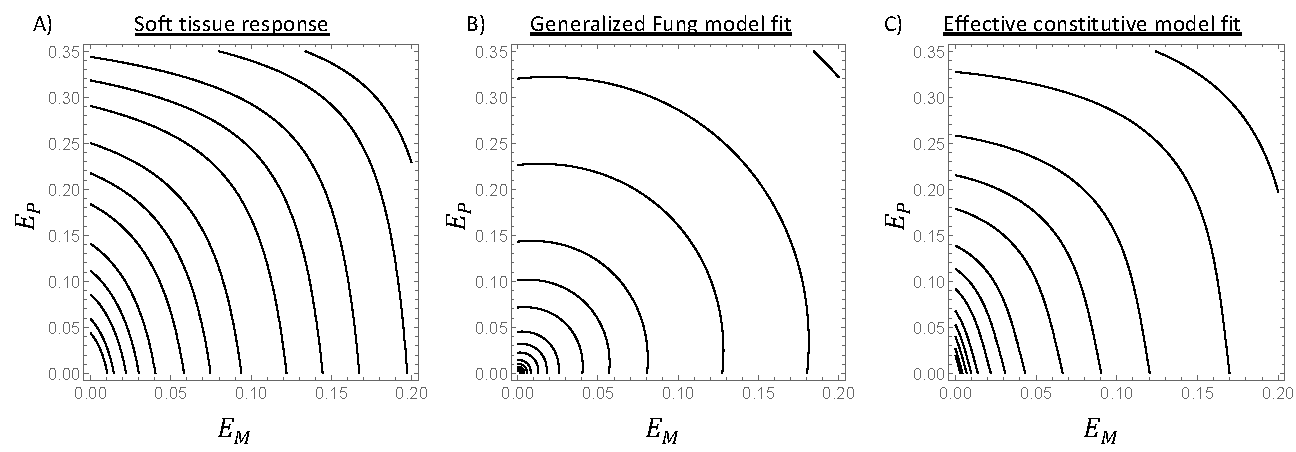
\includegraphics[width=\textwidth]{Images/chapter5/strainenergycontours}
\caption{The contour plots of strain energy (kPa) of A) a bovine pericardial specimen using a meso-scale structural model \cite{zhang_modeling_2017}, B) best fit using the generalized Fung model (Eqn. \ref{eqn:generalizedfungmodel}), and C) best fit using the effective constitutive model we develop from herein showing the necessity of extending existence phenomenological model form.}
\label{fig:strainenergycontours}
\end{figure}
%-------------------	 end FIGURE 	-------------------%
%%%%%%%%%%%%%%%%%%%%%%%%%%%%%%%%%%%%%%%%%%%%%%%%%%%%%%%%%%%%

\subsubsection{Final effective material model form} \label{sec:finalform}

	Thus, for the effective constitutive model, we extended the polynomial $Q$ one step further, allowing hyperellipticity of the strain energy density function (Fig. \ref{fig:strainenergycontours}C). For the additional terms to include, we move up to the next even powers, up to the quartic terms (exponents $i+j+k\leq4$) (Eqn. \ref{eqn:exponentialmodelform}), as odd numbered powers alone do not yield elliptical functions. There are a total of 34 possible terms in Q. Not all terms are required or even admissible. Specifically, the following constraints are enforced on the model:
      
    \underline{Constraint 1}: \underline{The stress must be zero in the reference configuration}. Given that the stress is the gradient of $\Psi$, where is $\Psi^\prime = c_0 Q^\prime e^Q$, all terms in $Q^\prime$ must be zero at zero strain. This corresponds to all $i+j+k = 1$ terms being removed, leaving 31 terms remaining. 
      
    \underline{Constraint 2}: \underline{The response must be elliptic}. That is the shortest line inscribed on the strain energy function surface joining any two points must have a positive curvature. Keeping in mind that the generalized Fung model (Eqn. \ref{eqn:exponentialmodelform}) is already close to being sufficient at reproducing the response of many soft tissues we tested. We only want to extend this to be able to reproduce a wider range of soft tissue responses. Furthermore, in considerations of limiting the number of parameters, reducing parameter correlation, improving the conditioning of the constrained objective function surface, and that the non-elliptical terms must be small, we choose to forgo all $i+j+k = 3$ terms, leaving 21 terms remaining. 
      
    \underline{Constraint 3}: \underline{Response must be independent of the direction of shear}. Since we decompose the Green-Lagrange strain relative to the material axis, this creates a plane of symmetry in the soft tissue response for the direction of shear. Thus, the value of $E_\phi$ can only have even powers, $k = 2,4$. The following terms are thus necessarily zero: $E_m^3E_\phi$, $E_m^2E_nE_\phi$, $E_mE_n^2E_\phi$, $E_n^3E_\phi$, $E_mE_\phi^3$, $E_nE_\phi^3$, $E_mE_\phi$, and $E_nE_\phi$. 
      
The final form of the effective constitutive model is thus
%==========================================================%
%-------------------	begin EQUATION 	-------------------%
\begin{equation}
\begin{aligned}\label{eqn:generalizeexponentialform}
\Psi	=& c_0 \left(e^{Q} - 1\right) \\
Q		=& b_1 E_m^2 + b_2 E_n^2 + b_3 E_\phi^2 + b_4 E_m E_n + b_5 E_m^4 + b_6 E_n^4 + b_7 E_m^3 E_n + b_8 E_m^2 E_n^2 + b_9 E_m E_n^3	\\
	&+ b_{10} E_\phi^4 + b_{11} E_m^2E_\phi^2 + b_{12} E_n^2 E_\phi^2 + b_{13} E_m E_n E_\phi^2.
\end{aligned}
\end{equation}
%-------------------	 end EQUATION 	-------------------%
%==========================================================%








%-----------------------------------------------------------
%	Model convexity
%-----------------------------------------------------------
\subsubsection{Enforcing convexity and ellipticity}

	Perhaps the biggest advantage of the single exponential approach models is the convenience for enforcing ellipticity and convexity. Because ellipticity and convexity are preserved by monotonically increase functions, such as $e^x$, we only have to enforce ellipticity and convexity of $Q$ (Eqn. \ref{eqn:generalizeexponentialform}). For strong ellipticity, the following must be satisfied,
%==========================================================%
%-------------------	begin EQUATION 	-------------------%
\begin{equation}\label{eqn:strongellipticity}
\dmd{\Psi}{2}{F_{ij}}{}{F_{kl}}{}\lambda_i\lambda_k\mu_j\mu_l > 0 \equiv \dmd{Q}{2}{F_{ij}}{}{F_{kl}}{}\lambda_i\lambda_k\mu_j\mu_l > 0,
\end{equation}
%-------------------	 end EQUATION 	-------------------%
%==========================================================%	
	where $F$ is any tensor, and $\lambda$ and $\mu$ are arbitrary non-zero vectors. \emph{This condition is also equivalent of strict convexity \cite{ball_strict_1980}}, so both conditions will be satisfied. Satisfying this constraint requires that the elasticity tensor $C_{ijkl}=\dmd{\Psi}{2}{E_{ij}}{}{E_{kl}}{}$ is positive definite, or rather $\dmd{Q}{2}{E_{ij}}{}{E_{kl}}{}$ is positive definite, satisfying Drucker stability for numerical purposes. Sylvester's criterion \cite{gilbert_positive_1991}, is the most convenient in this scenario, which is given by 
%==========================================================%
%-------------------	begin EQUATION 	-------------------%
\begin{equation}\label{eqn:convexitycriteria}
\begin{aligned}
&\dpd[2]{Q}{E_m} \geq 0, \quad
\det
\begin{bmatrix}
\dpd[2]{Q}{E_m} & \dmd{Q}{2}{E_m}{}{E_n}{}\\
\dmd{Q}{2}{E_m}{}{E_n}{} & \dpd[2]{Q}{E_n}\\
\end{bmatrix} \geq0, \quad  \\
&\det
\begin{bmatrix}
\dpd[2]{Q}{E_m} & \dmd{Q}{2}{E_m}{}{E_n}{} & \dmd{Q}{2}{E_m}{}{E_\phi}{}\\
\dmd{Q}{2}{E_m}{}{E_n}{} & \dpd[2]{Q}{E_n} & \dmd{Q}{2}{E_n}{}{E_\phi}{}\\
\dmd{Q}{2}{E_m}{}{E_\phi}{} & \dmd{Q}{2}{E_n}{}{E_\phi}{} & \dpd[2]{Q}{E_\phi} \\
\end{bmatrix} \geq0.
\end{aligned}
\end{equation}
%-------------------	 end EQUATION 	-------------------%
%==========================================================%
     For the generalized Fung model (Eqn. \ref{eqn:generalizedfungmodel}), $b_1>0$, $b_1b_2-b_4>0$, and $b_3(b_1b_2 - b_4^2) - b_5(b_2b_5 - b_4b_6) - b_6(b_1b_6 - b_4b5)>0$ will enforce convexity everywhere. For equation \ref{eqn:generalizeexponentialform}, this is slightly more complex. The non-convex region starts from a point along the respective axis for each component $E_m$, $E_n$, and $E_\phi$, then spreads out in the shape of a fan as the strain increases depending on which specific coupling terms, such as $E_m^3 E_n$ and $E_m E_n^3$ are present (Fig. \ref{fig:convexitybehavior}). As long as the effective constitutive model is convex on the largest value along the $E_m$, $E_n$, and $E_\phi$ axis respectively, then the effective constitutive model is convex over the entire range. For example, the effective constitutive model is convex if the maximum point on the $E_m$-axis is convex for $E_m^3 E_n$ (Fig. \ref{fig:convexitybehavior}A) or if the maximum point on the $E_n$-axis is convex for $E_m E_n^3$ (Fig. \ref{fig:convexitybehavior}B). Thus, assuming an upper limit of $E_m < 1$, $E_n < 1$, and $E_\phi < 1$, the following constraints on the parameters are sufficient to guarantee convexity and ellipticity,
%==========================================================%
%-------------------	begin EQUATION 	-------------------%
\begin{equation} \label{eqn:effmodelconstraints}
\begin{aligned}
b_1, b_2,b_3,b_5,b_6,b_{10} \geq 0	\\
4(b_1 + 6 b_5) (b_2 + b_8) - (b_4 + 3 b_7)^2 \geq 0		\\
4(b_2 + 6 b_6) (b_1 + b_8) - (b_4 + 3 b_9)^2 \geq 0 	\\
4(b_1 + b_{11}) (b_2 + b_{12}) - (b_{13} + b_4)^2 \geq 0 	\\
b_3+b_{11} \geq 0	\\
b_3+b_{12} \geq 0.	\\
\end{aligned}
\end{equation}
%-------------------	 end EQUATION 	-------------------%
%==========================================================%


%%%%%%%%%%%%%%%%%%%%%%%%%%%%%%%%%%%%%%%%%%%%%%%%%%%%%%%%%%%%
%-------------------	begin FIGURE 	-------------------%
\begin{figure}
\centering
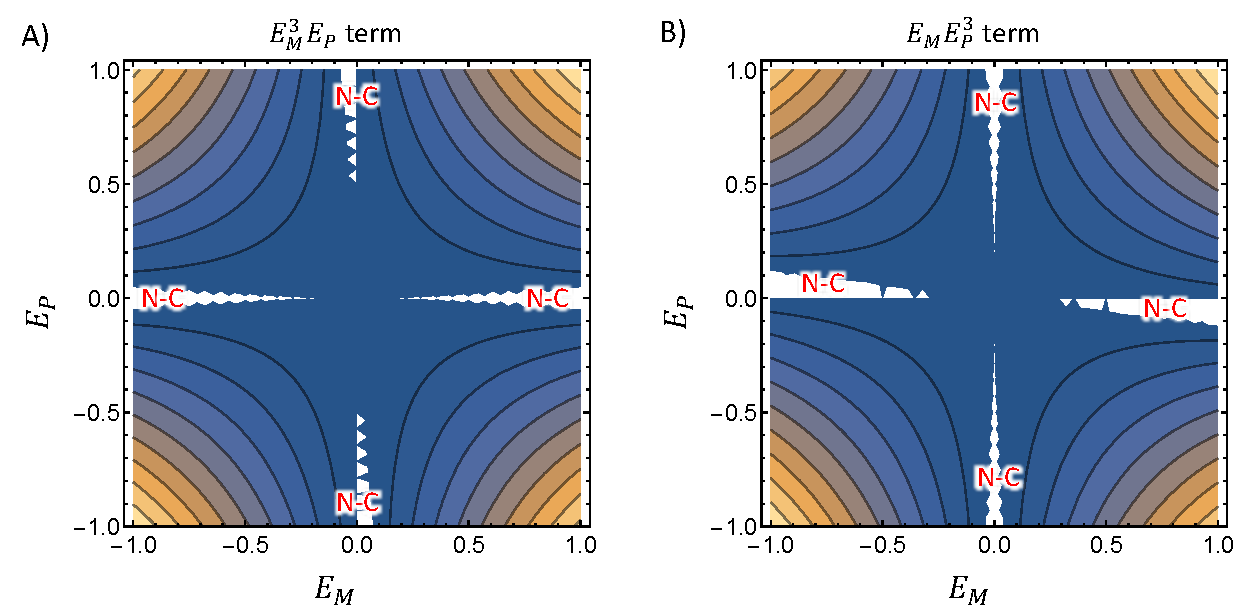
\includegraphics[width=\textwidth]{Images/chapter5/convexitybehavior}
\caption{The criteria for ellipticity (Eqn. \ref{eqn:convexitycriteria}) plotted against the components of the Green-Lagrange strain for A) when including the $E_m^3E_n$ term and B) $E_mE_n^3$ term. The white regions are not convex (N-C), which start at a point along the axes and spreads out as the strain increases.}
\label{fig:convexitybehavior}
\end{figure}
%-------------------	 end FIGURE 	-------------------%
%%%%%%%%%%%%%%%%%%%%%%%%%%%%%%%%%%%%%%%%%%%%%%%%%%%%%%%%%%%%










    
%-----------------------------------------------------------
%	Model scaling for parameter estimation
%-----------------------------------------------------------
\subsection{Model scaling method to improve parameters correlation for parameter estimation} \label{sec:modelscaling}

%-----------------------------------------------------------
%	Computational approaches	
\subsubsection{Parameter correlation for exponential type models}

	One challenging problem with model parameter determination is covariance between the parameters during parameter estimation. Covariance explains how two parameters influence the response of the model and how they will be updated during parameter estimation. High parameter covariance results in both slow convergence and poor reliability and reproducibility of the material parameters. When scaled by the variance, this becomes the correlation between the parameters, with an absolute value between $0$ and $1$. Correlation equal to $1$ implies that two parameters have the exact same effect on the model response, and are thus indistinguishable during parameter estimation. The covariance issue for constitutive models with an exponential function is well described by Aggarwal \cite{aggarwal_inverse_2015, aggarwal_improved_2017}. These constitutive models with exponential functions have a long valley like region in the objective function space. Inside this valley, significantly different parameters produce similar objective function values. This presents several problems. 1) It's difficult to compare model parameters between different specimens, because drastically different parameters can produce similar responses. As such, the average or representative specimen has little real meaning, and each specimen needs to be fitted individually for simulations. 2) The convergence of gradient based optimization algorithms becomes excruciatingly slow due to the small gradients while trapped within this valley. 3) The covariance between parameters being extremely large decreases the accuracy or in other word increases the confidence interval of parameters obtained. 
    
    Aggarwal \textit{et al.} suggested two improvements to alleviate this problem \cite{aggarwal_improved_2017}. These improvements are 1) modifying the modulus parameter $A$ to $e^{a}$, straightening the shape of the valley, and 2) introducing the log-norm for the objective function, improving the gradient along the valley. These modifications have been shown to be effective. However, this is not always ideal. The suggested logarithmic norm faces some issues when fitting stresses or strains, which may be negative and thus becomes undefined. Although this may be alleviated by forgoing data points with negative strains or stresses, but the model may still produce negative values during parameter estimation. Other methods can be used to discard negative values or to take the norm of such values, but these approaches create discontinuities in the gradient of the objective function, causing convergence problems during parameter estimation. Clearly, additional improvements can still be made. 


%-----------------------------------------------------------
%	Scaling method
\subsubsection{Model scaling method}

	We begin by examining the fundamental reason for the high parameter covariance. For this, we will use the 1-D case as an example,
%==========================================================%
%-------------------	begin EQUATION 	-------------------%
\begin{equation}
\begin{aligned}
\Psi &= A \left(e^{B \epsilon} - 1\right) \\
\mathcal{F} &= \sum_i \left(\Psi(\epsilon_i) - \Psi_i \right)^2,
\end{aligned}
\end{equation}
%-------------------	 end EQUATION 	-------------------%
%==========================================================%
where $\Psi$ is the strain energy of our model, $\epsilon$ is some invariant that is a function of the strain, $\epsilon_i$ and $\Psi_i$ are simulated data, and $\mathcal{F}$ is our objective function for parameter estimation. The parameters $A$ and $B$ have different purposes: $A$ is like a modulus, linearly increasing the stiffness of the material, while $B$ modifies the shape of the response, controlling the nonlinearity of the material. However, practically, the two parameters have nearly the same effect on the mechanical response, increasing $A$ increases the stiffness (Fig. \ref{fig:scalingapproach}A) and increasing $B$ also increases the stiffness (Fig. \ref{fig:scalingapproach}B). This is the reason for the high correlation between the parameters (Fig. \ref{fig:scalingapproach}), 0.9979.


%%%%%%%%%%%%%%%%%%%%%%%%%%%%%%%%%%%%%%%%%%%%%%%%%%%%%%%%%%%%
%-------------------	begin FIGURE 	-------------------%
\begin{figure}
\centering
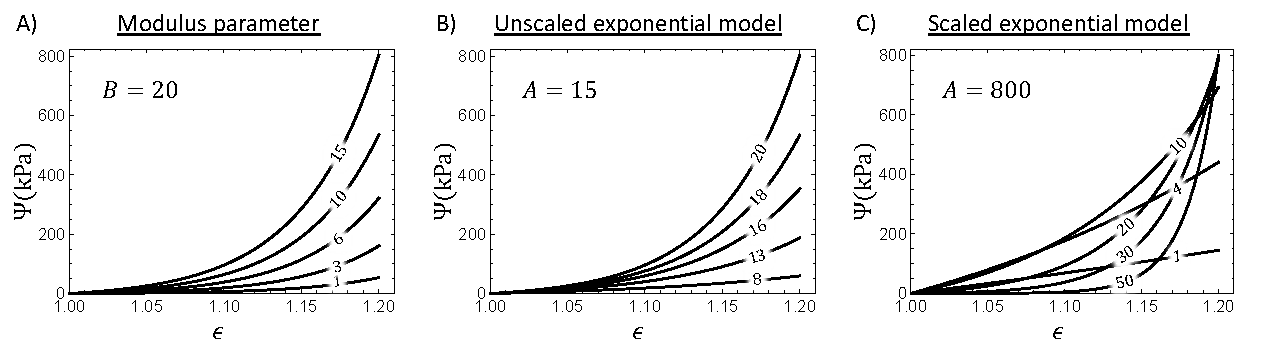
\includegraphics[width=\textwidth]{Images/chapter5/scalingapproach}
\caption{A)The effect of increasing the values of the modulus $A$ on exponential type models. B) The effect of increasing the values of exponent $B$ on exponential type models, which is nearly indistinguishable to the modulus $A$. C) The effect of increasing the values of parameter $B$ after applying the proposed scaling, increasing the values of parameter $A$ remains the same as in A).}
\label{fig:scalingapproach}
\end{figure}
%-------------------	 end FIGURE 	-------------------%
%%%%%%%%%%%%%%%%%%%%%%%%%%%%%%%%%%%%%%%%%%%%%%%%%%%%%%%%%%%%


	To address this problem, we introduce a scaling term to normalize the exponential part of the model. This prevents increasing $B$ from increasing the value of the strain energy as a whole, allowing it to only control the curvature. For this, we will use a value $\epsilon_{max}$, which represents the data point with the maximum strain energy value used for parameter estimation, which is also the point where the strain energy stays constant with changes in $B$. The scaled form is thus given by
%==========================================================%
%-------------------	begin EQUATION 	-------------------%
\begin{equation}
\begin{aligned}
\Psi = \Psi_s = \bar{A} \left[e^{-B\epsilon_{max}} \left( e^{B\epsilon} - 1\right)\right],\label{eqn:scaledmodel1D}
\end{aligned}
\end{equation}
%-------------------	 end EQUATION 	-------------------%
%==========================================================%
    where $\bar{A}$ is the scaled version of the modulus $A$. This scaling keeps the exponential part of the model, $e^{-B\epsilon_{max}} ( e^{B\epsilon} - 1)$, at approximately 1.0 at $\epsilon = \epsilon_{max}$, regardless of the changes in the value of the parameter $B$ (Fig. \ref{fig:scalingapproach}C). This effect is not exact when the value of $B$ is small due to the $-1$ needed to set the strain energy to 0 in the referential configuration, but is nonetheless sufficient for our goal: decoupling the modulus increasing effect of the parameter $A$ from the curvature increasing effect of parameter $B$. Indeed, we found this approach to be successful. We examined the contour plot of the objective function with respect to each of the 4 cases in Aggarwal's work \cite{aggarwal_improved_2017}, with the standard objective function, with $A=e^{a}$, with log-norm, and with $A=e^{a}$ and the log-norm, for both without scaling and with scaling (Fig. \ref{fig:objfunctionsurfaces}). First, the correlation between the parameters does not change with $A=e^{a}$. The log-norm improves the correlation from 0.9979 to 0.9063 (Table \ref{tb:ABcorrelation}), which significantly improves the objective function surface (Fig. \ref{fig:objfunctionsurfaces}). On the other hand, our scaling method improves the correlation from 0.9979 to 0.6186, more significant than using the log-norm. Interestingly, combining scaling and the log-norm has the adverse effect, increasing the correlation back from 0.6186 to 0.8592. This is a result of essentially linearizing the relation between $A$ and $B$, i.e. from $Ae^{B\epsilon}$ to $Log(A)+B\epsilon$, causing the relationship between $A$ and $B$ to go from modulus and nonlinearity to baseline and modulus. Clearly, \emph{the most optimal parameter estimation approach is to use scaling method with no other modifications}. 
    
    
%%%%%%%%%%%%%%%%%%%%%%%%%%%%%%%%%%%%%%%%%%%%%%%%%%%%%%%%%%%%
%-------------------	begin FIGURE 	-------------------%
\begin{figure}
\centering
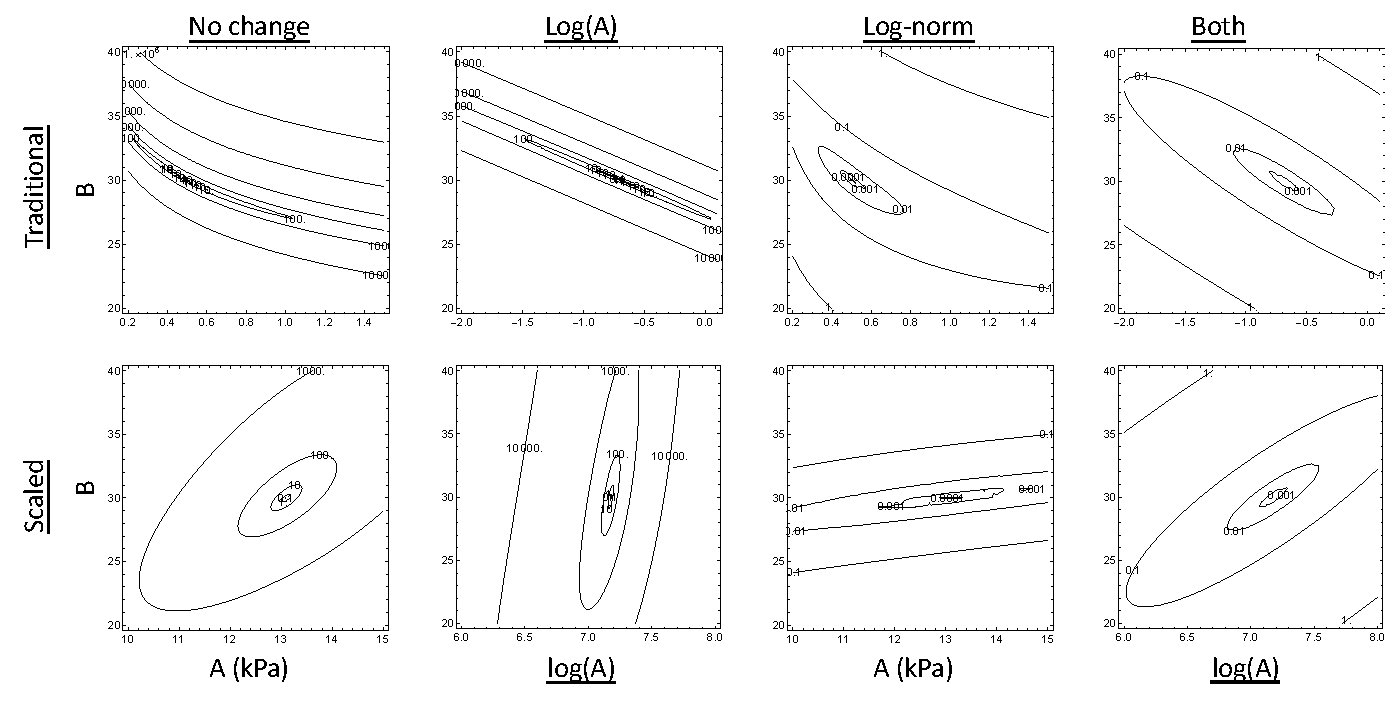
\includegraphics[width=\textwidth]{Images/chapter5/objfunctionsurfaces}
\caption{(Top) The objective function surface for the traditional unscaled exponential models and (Bottom) objective function surface after scaling. From Left to Right are: the unchanged surface, the surface after changing $A$ to $e^{a}$, using the log-norm for the objective function, and applying both changes. The scaled form with no other changes behaves the best.}
\label{fig:objfunctionsurfaces}
\end{figure} 
%-------------------	 end FIGURE 	-------------------%
%%%%%%%%%%%%%%%%%%%%%%%%%%%%%%%%%%%%%%%%%%%%%%%%%%%%%%%%%%%%


%----------------------------------------------------------%
%-------------------	begin TABLE 	-------------------%
\begin{table}
\caption{The correlation between model parameter when using Hencky strains}
\begin{center}
\label{tb:ABcorrelation}
\begin{tabular}{|l|rrrr|}
\hline
			& No change	& $\log(A)$	& $\log$-norm	& Both \\
\hline
Traditional	& -0.9979	& -0.9979	& -0.9063		& -0.9063 \\
Scaled 		& 0.6186	& 0.6186	& 0.8592		& 0.8592 \\
\hline
\end{tabular}
\end{center}
\end{table}
%-------------------	 end TABLE 		-------------------%
%----------------------------------------------------------%



%-----------------------------------------------------------
%	Relation to unscaled form
% \subsubsection{Relation to unscaled model}

    By design, the value of the exponential parameter $B$ does not change by using the scaling method. Since the scaling term does not depend on the input strain, it acts as a modification to the modulus $A$ while keeping the exponential term the same. This also implies that the relationship between the unscaled modulus $A$ and the scaled modulus $\bar{A}$ is
%==========================================================%
%-------------------	begin EQUATION 	-------------------%
\begin{equation}
\begin{aligned}
A = \bar{A} e^{-B\epsilon_{max}},
\end{aligned}
\end{equation}
%-------------------	 end EQUATION 	-------------------%
%==========================================================%
which makes finding the actual unscaled parameters a simple task. One other benefit of this scaling approach is that the value of $\bar{A}$ is extremely straight forward and intuitive, it is the strain energy of the model at $\epsilon_{max}$. As a result, the value of $\bar{A}$ can be determined \textit{a priori}, or at the very least it is easy to make an initial guess for $\bar{A}$. This will in turn also help to make parameter estimation faster and more accurate, leaving only the parameter $B$ to be determined. 


%-----------------------------------------------------------
%	Extension to multi-variable form
\subsubsection{Extension to multiple variables}

	Extending this method to multiple variables is very simple. For $\Psi_{eff}$ (Eqn. \ref{eqn:generalizeexponentialform}), the input variables become $\mathbf{\epsilon} = \{E_m, E_n, E_\phi\}$, and $\mathbf{\epsilon}_{max} = \{E_m^{max},E_n^{max},E_\phi^{max}\}$. Determining the values for $\mathbf{\epsilon}_{max}$ depends on the form of the objective function. Using the most common case as the example, which is the sum of the squares of the differences in the 2nd Piola Kirchhoff stress,
%==========================================================%
%-------------------	begin EQUATION 	-------------------%
\begin{equation}
\begin{aligned}
\mathcal{F} = \sum_i \left(S_{11}(\epsilon_i) - \hat{S}_{11}^i\right)^2 + \left(S_{12}(\mathbf{\epsilon}_i) - \hat{S}_{12}^i\right)^2 + \left(S_{22}(\epsilon_i) - \hat{S}_{22}^i\right)^2,
\end{aligned}
\end{equation}
%-------------------	 end EQUATION 	-------------------%
%==========================================================%
$\mathbf{\epsilon}_{max}$ is the data point $\mathbf{\epsilon}_i$ which maximizes $\left(\hat{S}_{11}^i\right)^2 + \left(\hat{S}_{12}^i\right)^2 + \left(\hat{S}_{22}^i\right)^2$. 
Thus, we also introduce a $Q_{max}$ such that,
%==========================================================%
%-------------------	begin EQUATION 	-------------------%
\begin{equation} \label{eqn:finalexponentialmodelformscaled}
\begin{aligned}
\Psi_{eff} 	=& c_0 \left(e^{Q} - 1\right) = c_0^\prime e^{-Q_{max}}\left(e^{Q} - 1\right)    \\
Q		=& b_1 E_m^2 + b_2 E_n^2 + b_3 E_\phi^2 + b_4 E_m E_n + b_5 E_m^4 + b_6 E_n^4 + b_7 E_m^3 E_n + b_8 E_m^2 E_n^2 \\ 
&+ b_9 E_m E_n^3 + b_{10} E_\phi^4 + b_{11} E_m^2E_\phi^2 + b_{12} E_n^2 E_\phi^2 + b_{13} E_m E_n E_\phi^2 \\
Q		=& b_1 (E_m^{max})^2 + b_2 (E_n^{max})^2 + b_3 (E_\phi^{max})^2 + b_4 (E_m^{max}) (E_n^{max}) + b_5 (E_m^{max})^4   \\
    &+ b_6 (E_n^{max})^4 + b_7 (E_m^{max})^3 (E_n^{max}) + b_8 (E_m^{max})^2 (E_n^{max})^2 + b_9 (E_m^{max}) (E_n^{max})^3	\\
	&+ b_{10} (E_\phi^{max})^4 + b_{11} (E_m^{max})^2(E_\phi^{max})^2 + b_{12} (E_n^{max})^2 (E_\phi^{max})^2    \\ 
	&+ b_{13} (E_m^{max}) (E_n^{max}) (E_\phi^{max})^2,
\end{aligned}
\end{equation}
%-------------------	 end EQUATION 	-------------------%
%==========================================================%
where parameter estimation will be done for $c_0^\prime$ instead of $c_0$. Computing the response functions and the stresses, or even the elasticity tensor remains very simple, only requiring multiplying each term by $e^{-Q_{max}}$. Thus, this scaling method is a very simple and easy to implement method of improving the speed and convergence for the parameter estimation of exponential type models. 












%-----------------------------------------------------------
%	Optimal loading paths
%-----------------------------------------------------------
\subsection{Optimal \textit{in silico} loading paths for parameter estimation}\label{sec:optimaldesign}

	Another technique for improving the parameter estimation process for determining $\Psi_{eff}$ from respective micro-models is establishing optimal loading paths. An example is the work of Avazmohammadi \cite{avazmohammadi_novel_2017}, where optimal experimental design is used to 1) minimize the amount of data necessary and 2) improve model parameter covariance for parameter estimation. Just like one of the most important question to ask before performing any mechanical testing is how much and what kind of data is necessary, we should also be selective with our choice of sampling points for parameter estimation. The theory for optimal design of experiment is well-studied and documented \cite{lanir_optimal_1996, zhu_d_2014}. Vast majority of the methods for optimal design uses D-optimality as the design variable,
%==========================================================%
%-------------------	begin EQUATION 	-------------------%
\begin{equation}\label{eqn:doptimality}
\begin{aligned}
D = \det(\mathbfcal{I}), \quad \mathbfcal{I} = \mathbf{J}^\mathsf{T}\mathbf{J} \quad \mathrm{or} \quad \mathbfcal{I} = \mathbfcal{H},	\\
\mathrm{where} \ J_{ij} = \dpd{f_i}{\xi_j}, \quad \mathcal{H}_{ij} = \dmd{\mathcal{F}}{2}{\xi_i}{}{\xi_j}{},
\end{aligned}
\end{equation}
%-------------------	 end EQUATION 	-------------------%
%==========================================================% 
    where $\mathbf{\xi}$ is a vector of model parameters and $\mathbfcal{I}$ is the information matrix. $\mathbfcal{I}$ can be computed from the derivatives of the objective function $\mathcal{F}$, where $f$ is the model evaluated at each data point, or it can be computed from the Hessian of the objective function, $\mathbfcal{H}$ (Appendix \ref{sec:parametercorrelation}). D-optimality is the determinant of the information or the hessian matrix at the best fit value. It offers the best representation of both parameter accuracy (parameter covariance or correlation) and precision (parameter variance) at the same time.

    
    The first and foremost step is to establish the parameterization for loading paths so they can be optimized. This is not a straightforward choice, as the number of loading path required is not yet established. Another issue is that the number of data points is discrete, thus the gradient of the D-optimality with respect to the control parameters is not smooth. For the sake of time spent for optimization, the number of data points should be kept as small as possible, thus exacerbating the issue of differentiability. Even worse is perhaps that the objective function is essentially flat when not near the optimum, making gradient algorithms not practical. Monte Carlo, random search or divide and conquer strategies are needed, which are much more time consuming. The search space also increases exponentially with the number of loading paths, making a fully exhaustive search difficult to implement. Thus, a simple parameterization for loading paths is ideal. 
    

%%%%%%%%%%%%%%%%%%%%%%%%%%%%%%%%%%%%%%%%%%%%%%%%%%%%%%%%%%%%
%-------------------	begin FIGURE 	-------------------%
\begin{figure}
\centering
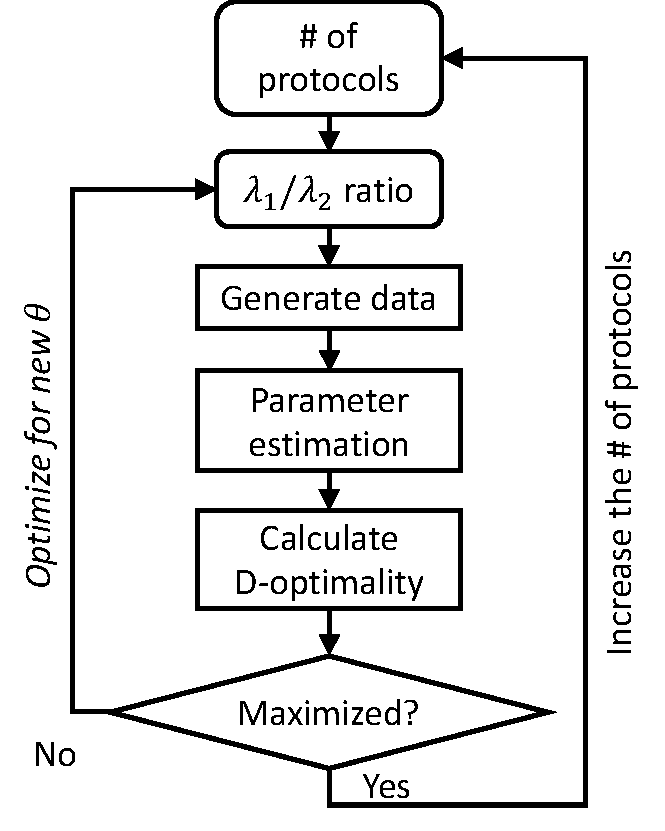
\includegraphics[width=2.5in]{Images/chapter5/optimaldesign}
\caption{Our approach for optimizing for the optimal loading paths for parameter estimation.}
\label{fig:optimaldesign}
\end{figure}
%-------------------	 end FIGURE 	-------------------%
%%%%%%%%%%%%%%%%%%%%%%%%%%%%%%%%%%%%%%%%%%%%%%%%%%%%%%%%%%%%

    
    We define loading paths based on the following conditions: 
\begin{enumerate}
\item The number of loading paths is as small as possible
\item The number of variables needed to define a loading path is as small as possible
\item Possible application to mechanical testing of tissues.
\end{enumerate} 
    Starting with planar extensions only, we chose a loading path as data points which shares the same stretch ratio, $\lambda_1/\lambda_2$, which is typically the same definition used for biaxial mechanical testing. This only requires one constant to be defined for each loading path and the resulting fan shape covers the largest range of deformation with the least number of data points. To determine the optimal loading paths, 1) the total number of loading paths was set, then 2) each combination of the stretch ratios was evaluated for the highst D-optimality (Fig. \ref{fig:optimaldesign}). For a total number of loading paths ranging from 1 to 6, we found the the point when the D-optimality stops increasing significantly, and choose this as the optimal set. Next the shear component, $\kappa_1$, is added. For this study, we constrained the shear to be $0<\kappa_1<0.2$. Only the positive values of $\kappa_1$ is allowed due to the material symmetry. Furthermore, the optimal planar extensions loading paths are always included as a part of the data set.














%%%%%%%%%%%%%%%%%%%%%%%%%%%%%%%%%%%%%%%%%%%%%%%%%%%%%%%%%%%%%
%%  Model Applications										%
%%%%%%%%%%%%%%%%%%%%%%%%%%%%%%%%%%%%%%%%%%%%%%%%%%%%%%%%%%%%%

%-----------------------------------------------------------
%	Use of structural constitutive models
%-----------------------------------------------------------
\subsection{Example application for planar soft tissues}

	The exogenously cross-linked structural model presented in Zhang and Sacks \cite{zhang_modeling_2017} is used to test our approach (Fig. \ref{fig:simulationframework}) and see if $\Psi_{eff}$ (Eqn. \ref{eqn:finalexponentialmodelformscaled}) can completely reproduce its response. This meso-scale structural model is computationally expensive due to integration over the collagen fiber architecture but have been shown to be able to accurately reproduce the mechanical response of a variety of soft tissues, such as mitral valve leaflets \cite{zhang_meso_2016}, ovine pulmonary artery \cite{fata_insights_2014}, myocardium \cite{avazmohammadi_novel_2017}, and exogenously cross-linked bovine pericaridium \cite{sacks_novel_2016}. To briefly summarize, this model is composed of 3 components: collagen, $\Psi_\mathrm{col}$, matrix, $\Psi_\mathrm{mat}$, and interactions, $\Psi_\mathrm{int}$. 
%==========================================================%
%-------------------	begin EQUATION 	-------------------%
\begin{equation}
\Psi 	= \Psi_\mathrm{col} + \Psi_\mathrm{mat} + \Psi_\mathrm{int} \label{eqn:structuralmodelcomponents}
\end{equation}
%-------------------	 end EQUATION 	-------------------%
%==========================================================%
    The matrix term, $\Psi_\mathrm{mat}$, is a modified version of the Yeoh model that is more linear when expressed in 2nd Piola Kirchhoff stress versus stretch, 
%==========================================================%
%-------------------	begin EQUATION 	-------------------%
\begin{equation}\label{eqn:matrixmodel}
\begin{aligned}
\Psi_\mathrm{mat} = &\frac{\eta_M}{2} \left[ \frac{1}{a}\left( I_1 -3\right)^{a} + \frac{r}{b} \left( I_1 -3\right)^{b} \right], \\
&\text{with } 1<a<b, ab <2, 0 \leq r.
\end{aligned}
\end{equation}
%-------------------	 end EQUATION 	-------------------%
%==========================================================%
    This model contains four parameters: $\eta_M$ is the modulus parameter corresponding to the same parameter in the Neo Hookean model, $a$, $b$, and $r$ are the shape parameters, where $a$ and $b$ control the shape of the two terms, while $r$ is the weight between the two terms. In general, $a \approx 1$, $b \approx 1.87$ and $r \approx 15$ can be treated as constants. 


	The response of collagen fibers is given by the integration over the collagen fibers architecture, their orientation and crimp. The fiber orientations is described by a beta distribution function and fiber crimp is described by another beta distribution function of the stretches needed to straighten the fibers, the slack stretch $\lambda_s$. These are referred to as the orientation distribution function (ODF), $\Gamma$, and the recruitment distribution function (RDF), $D$, respectively, with the forms given in Zhang and Sacks \cite{zhang_meso_2016, zhang_modeling_2017, sacks_novel_2016}. The form of the strain energy function is 
%==========================================================%
%-------------------	begin EQUATION 	-------------------%
\begin{equation} \label{eqn:collagen}
\begin{aligned}
\Psi_\mathrm{col} =& \phi_\mathrm{col} \eta_C \int\displaylimits_\theta \Gamma(\theta) 
\int\displaylimits_1^{\lambda_\theta} D\left(\lambda_s \right) \left( \frac{\lambda_\theta}{\lambda_s} - 1\right)^2 \mathrm{d}\lambda_s \mathrm{d}\theta,
\end{aligned}
\end{equation}
%-------------------	 end equation 	-------------------%
%----------------------------------------------------------%
    where $\eta_C$ is the modulus of the collagen fibers, $\lambda_\theta = \sqrt{\mathbf{n}_\theta \cdot \mathbf{C}\mathbf{n}_\theta}$ is the stretch of the ensemble of collagen fiber with the same orientation, and $\lambda_\mathrm{\theta}/\lambda_s$ is the true stretch of the collagen fibers after they are straightened \cite{zhang_meso_2016}. Similarly, the response of the interaction term is given by integration over pairs of fibers based on their orientation and crimp, which contains a quadruple integral. 
%==========================================================%
%-------------------	begin EQUATION 	-------------------%
\begin{equation}
\Psi_\mathrm{int} = \frac{\eta_I}{2} \int\displaylimits_\alpha \int\displaylimits_\beta \Gamma(\alpha) \Gamma(\beta) \int\displaylimits_1^{\lambda_\alpha} \int\displaylimits_1^{\lambda_\beta} D\left( x_\alpha \right) D\left( x_\beta \right) \left( \frac{\lambda_\alpha \lambda_\beta}{x_\alpha x_\beta} - 1\right)^2 \,\mathrm{d}x_\alpha \,\mathrm{d}x_\beta \,\mathrm{d}\alpha \,\mathrm{d}\beta.
\end{equation}
%-------------------	 end EQUATION 	-------------------%
%==========================================================%
For clarity of presentation, the slack stretches, $\lambda_s$, are replaced by $x_\alpha$ and $x_\beta$ for fiber oriented along the angle $\alpha$ and $\beta$ respectively. Only one parameter, the modulus $\eta_I$, is used to account for all interactions, with the same $\Gamma$ and $D$ already given above. 

The second Piola Kirchhoff stress, $\mathbf{S}=2\frac{\partial\Psi}{\partial\mathbf{C}}$, is 
%==========================================================%
%-------------------	begin EQUATION 	-------------------%
\begin{equation} \label{eqn:fullcollagen}
\begin{aligned}
\mathbf{S} = & \phi_\mathrm{col} \eta_C \int\displaylimits_\theta \Gamma(\theta)\left\lbrace 
\int\displaylimits_1^{\lambda_\theta} \frac{D\left( x \right)}{x} \left( \frac{1}{x}- \frac{1}{\lambda_\theta}\right) \mathrm{d}x \right\rbrace \mathbf{n}_\theta\otimes\mathbf{n}_\theta \mathrm{d}\theta \\
+ & \phi_\mathrm{col} \eta_I \int\displaylimits_\alpha \int\displaylimits_\beta \Gamma \left(\alpha \right) \Gamma \left( \beta \right) \\
& \times \left[ \left\lbrace 
\int\displaylimits_1^{\lambda_\alpha} \int\displaylimits_1^{\lambda_\beta} 
\frac{2 \lambda_\beta D(x_\alpha) D(x_\beta)}{x_\alpha x_\beta} 
\left( \frac{\lambda_\alpha}{x_\alpha} \frac{\lambda_\beta}{x_\beta} - 1\right) \mathrm{d}x_\alpha \, \mathrm{d}x_\beta\right.\right.   \\
&\quad\left.\left.+\int\displaylimits_1^{\lambda_\beta} D(x_\beta) \left( \frac{\lambda_\beta}{x_\beta} -1  \right)^2 \mathrm{d}x_\beta \right\rbrace \right.  \frac{\mathbf{n}_\alpha \otimes \mathbf{n}_\alpha}{\lambda_\alpha}  \\
& + \left. \left\lbrace
\int\displaylimits_1^{\lambda_\alpha} \int\displaylimits_1^{\lambda_\beta} 
\frac{2 \lambda_\alpha D(x_\alpha) D(x_\beta)}{x_\alpha x_\beta} 
\left( \frac{\lambda_\alpha}{x_\alpha} \frac{\lambda_\beta}{x_\beta} - 1\right) \mathrm{d}x_\alpha \, \mathrm{d}x_\beta\right.\right.   \\
&\quad \left.\left. + \int\displaylimits_1^{\lambda_\alpha} D(x_\alpha) \left( \frac{\lambda_\alpha}{x_\alpha} -1  \right)^2 \mathrm{d}x_\alpha \right\rbrace \frac{\mathbf{n}_\beta \otimes \mathbf{n}_\beta}{\lambda_\beta}  \right] \mathrm{d}\alpha \, \mathrm{d}\beta\\
+ & \phi_\mathrm{mat} \eta_M \left[\left(\left( I_1 - 3\right)^{a - 1} + r \left( I_1 - 3\right)^{b - 1}\right) \left( \mathbf{I} - C_{33}\mathbf{C}^{-1}\right)  \right],\\
\end{aligned}
\end{equation}
%-------------------	 end EQUATION 	-------------------%
%==========================================================%
    where $\phi_\mathrm{col}$ and $\phi_\mathrm{mat}$ are the mass fraction of collagen and matrix respectively. 
    
	Although this model is very accurate and predictive, it is also computationally expensive. Moreover, numerical integration results in a significant decrease in numerical precision when the number of quadrature point is insufficient. This can create a number of issues for convergence during parameter optimization. Thus, the implementation of this model is complicated by a constant balance between computational cost and numerical robustness during optimization. Using $\Psi_{eff}$ to reproduce its response is a solution to these issues. %Furthermore, some modifications can be made to reduce the form of $\psi_{eff}$ based on how well each term captures the behavior of the respective material (see Appendix \ref{sec:specificform}).
    
    
    



	









%-----------------------------------------------------------
%	Parameter estimation
%-----------------------------------------------------------
\subsection{Parameter estimation}

	The objective function we use is 
%==========================================================%
%-------------------	begin EQUATION 	-------------------%
\begin{equation}\label{eqn:objectivefunction}
\begin{aligned}
S_m =& \dpd{\Psi}{E_m} = \mathbf{m}_0\cdot\mathbf{S}\mathbf{m}_0,
	\  S_n = \dpd{\Psi}{E_n} = \mathbf{n}_0\cdot\mathbf{S}\mathbf{n}_0, 
    \  S_\phi = \dpd{\Psi}{E_\phi} = 2\mathbf{m}_0\cdot\mathbf{S}\mathbf{n}_0 \\
\mathcal{F} =& \sum_i^n \left(S_m(\hat{E}_M^i, \hat{E}_S^i, \hat{E}_\phi^i) - \hat{S}_M^i \right)^2 + \left(S_n(\hat{E}_M^i, \hat{E}_S^i, \hat{E}_\phi^i) - \hat{S}_S^i \right)^2     \\
    &+ \left(S_\phi(\hat{E}_M^i, \hat{E}_S^i, \hat{E}_\phi^i) - \hat{S}_\phi^i \right)^2
\end{aligned}
\end{equation}
%-------------------	 end EQUATION 	-------------------%
%==========================================================%
    This removes rigid body rotation and puts the stresses along the material axes, giving the response functions and minimizes covariance between the parameters during optimization. Other possible options include the log of the L2-norm, the log-norm presented by Aggarwal \cite{aggarwal_improved_2017}, and L2-norm of the strain energy and other stresses.


	For optimal speed, gradient methods are ideal. Because we require some non-linear constraints to enforce convexity, we utilized the interior point algorithm provided by the IPOPT library \cite{waechter_implementation_2005}. The initial guess is easily derived for the model scaling method, with the parameter $c_0$ being the maximum strain energy in the available data. The exponent parameters $b_i$ are generally very consistent in value, with the quadratic parameters being $b_1 \approx 10$, $b_2 \approx 10$, and $b_4 \approx -10$, the quartic parameters being $b_5 \approx 2000$, $b_6 \approx 500$, $b_9 \approx 200$, $b_{10} \approx 200$, $b_{11} \approx 200$, $b_{12} \approx 200$. We find this setup to work extremely well, and no further modifications are necessary. 




\subsection{Reproducing the response of soft tissues using the effective constitutive model and optimal loading paths}\label{sec:reproducefung}

	For our approach (Fig. \ref{fig:simulationframework}), we need to overcome the limitation of common phenomenological approaches on predicting the mechanical response of micro-models outside of the data set used for parameter estimation \cite{sun_biaxial_2003}. To verify this, we will first reproduced the results of Sun \textit{et al.} \cite{sun_biaxial_2003} using the generalized Fung model, then repeat the process using $\Psi_{eff}$ (Eqn. \ref{eqn:finalexponentialmodelformscaled}) with optimal loading paths. We will focus on glutaraldehyde cross-linked bovine pericardium as the tissue. Bovine pericardium is the most common material used to fabricate bioprosthetic heart valves. It is extremely dense in collagenous fibers, having broad fiber splays with approximately $30\deg$ in standard deviation. The resulting mechanical behavior have strong coupling between the axial stretches. Thus, the mechanical response of some bovine pericardium specimens are fitted to the structural model (Eqn. \ref{eqn:fullcollagen}). The structural model is then used to generate stress strain data along loading paths with stress ratios ($S_{11}/S_{22}$) of $0.1:1$, $0.5:1$, $0.75:1$, $1:1$, $1:0.75$, $1:0.5$, and $1:0.1$. Following Sun \textit{et al.} \cite{sun_biaxial_2003}, the generalized Fung model (Eqn. \ref{eqn:generalizedfungmodela}) was fitted to the five loading paths in the physiologic range ($0.5:1$, $0.75:1$, $1:1$, $1:0.75$, $1:0.5$), then the remaining two loading paths were predicted and compared to the data. Next, the reverse scenario was done, where the generalized Fung model was fitted to the non-physiologic loading paths ($0.1:1$ and $1:0.1$), while the remaining five loading paths were predicted. Following the same step, $\Psi_{eff}$ was fitted to the three optimal loading paths ($0.1:1$, $1:1$, and $1:0.1$) while the remaining loading paths were predicted. 
    
    We also considered some alternative loading paths. In the original paper by Fung et al. on the constitutive modeling of arteries \cite{fung_pseudoelasticity_1979}, they discussed the use of 'physiologic protocols' as the optimal data set for parameter estimation. These 'physiologic protocols' are loading paths that cover a range past some predetermined lower bounds for $E_{11}$ and $E_{22}$. Conceptually, this is meant to correspond to the range after accounting for the prestrain between the zero stress configuration and the \textit{in vivo} unloaded (not stress free) configuration. For clarity, to distinguish between this and the physiologic range (the range where the physiologic loading path is likely to reside) in Sun \textit{et al.}, we will refer to this as the prestrained range. We reproduced the prestrained protocols in figure 5 of Fung \textit{et al.} \cite{fung_pseudoelasticity_1979}, and compared the results to those with optimal loading paths. 






